\section{Résultats Expérimentaux}

Cette section présente les résultats des deux benchmarks : l'évaluation des
modèles d'embedding et la comparaison des stratégies de recherche.

\subsection{Benchmark des Modèles d'Embedding}

Le tableau~\ref{tab:embedding_results} présente les performances agrégées
des cinq modèles d'embedding sur le corpus de 26 articles juridiques avec
65 variantes de requêtes.

\begin{table}[H]
\centering
\caption{Résultats du benchmark des modèles d'embedding}
\label{tab:embedding_results}
\resizebox{\columnwidth}{!}{%
\begin{tabular}{lcccccc}
\toprule
\textbf{Modèle} & \textbf{P@1} & \textbf{P@3} & \textbf{P@5} & \textbf{MRR} & \textbf{NDCG} & \textbf{Acc. Dom.} \\
\midrule
E5-large (1024d) & 0,72 & 0,68 & 0,61 & 0,81 & 0,76 & 0,89 \\
BGE-M3 (1024d)   & 0,69 & 0,65 & 0,58 & 0,78 & 0,73 & 0,85 \\
LaBSE (768d)     & 0,61 & 0,58 & 0,52 & 0,70 & 0,66 & 0,78 \\
E5-base (768d)   & 0,58 & 0,54 & 0,49 & 0,67 & 0,63 & 0,74 \\
MPNet (768d)     & 0,52 & 0,49 & 0,45 & 0,61 & 0,58 & 0,68 \\
\bottomrule
\end{tabular}
}
\end{table}

\subsubsection{Analyse par Dimension}

Les modèles 1024 dimensions (E5-large, BGE-M3) surclassent significativement
les modèles 768 dimensions sur toutes les métriques. E5-large atteint le
meilleur MRR (0,81) et la meilleure précision de domaine (89\%). Cette
supériorité s'explique par la capacité des embeddings de plus haute dimension
à capturer les nuances fines du vocabulaire juridique arabe.

\subsubsection{Analyse par Type de Requête}

Le tableau~\ref{tab:embed_by_type} décompose les performances d'E5-large selon
le type de requête.

\begin{table}[H]
\centering
\caption{Performance de E5-large par type de requête}
\label{tab:embed_by_type}
\begin{tabular}{lcc}
\toprule
\textbf{Type de requête} & \textbf{P@1} & \textbf{MRR} \\
\midrule
Arabe formel (MSA)       & 0,91 & 0,94 \\
Arabe dialectal (Darija) & 0,65 & 0,73 \\
Mots-clés courts         & 0,72 & 0,79 \\
Cross-lingue français    & 0,78 & 0,85 \\
Cross-lingue anglais     & 0,81 & 0,88 \\
\bottomrule
\end{tabular}
\end{table}

Le \textbf{gap Darija--MSA} est significatif : 65\% contre 91\%, soit une
baisse relative de 29\%. Ce résultat confirme que la diglossie arabe constitue
un défi majeur pour les modèles d'embedding multilingues. Les requêtes
cross-lingues (français $\to$ arabe : 78\%, anglais $\to$ arabe : 81\%)
montrent une capacité de transfert inter-langue appréciable, cruciale dans
le contexte marocain où le code-switching arabe/français est courant.

\subsubsection{Débit d'Embedding}

Le tableau~\ref{tab:embed_speed} présente le débit d'embedding mesuré sur GPU
T4 (Google Colab) :

\begin{table}[H]
\centering
\caption{Débit d'embedding par modèle (GPU T4, batch 200 textes)}
\label{tab:embed_speed}
\begin{tabular}{lccc}
\toprule
\textbf{Modèle} & \textbf{Textes/s} & \textbf{Dim.} & \textbf{P@1} \\
\midrule
E5-base (fallback CPU) & 78 & 768 & 0,58 \\
MPNet                 & 72 & 768 & 0,52 \\
LaBSE                 & 65 & 768 & 0,61 \\
E5-large (production) & 42 & 1024 & 0,72 \\
BGE-M3                & 38 & 1024 & 0,69 \\
\bottomrule
\end{tabular}
\end{table}

E5-large offre le meilleur compromis (42 textes/s pour 72\% P@1). En mode CPU
(fallback), E5-base est l'alternative avec 78 textes/s.

\subsubsection{Significativité Statistique}

Des tests $t$ de Student appariés confirment que la différence entre E5-large
et BGE-M3 n'est pas statistiquement significative ($p = 0,08$), tandis que
les différences avec les modèles 768d le sont toutes ($p < 0,01$). Les deux
modèles 1024d sont donc interchangeables pour la production.

\subsection{Benchmark des Stratégies de Recherche}

Le tableau~\ref{tab:retrieval_results} présente les résultats sur 32
questions juridiques.

\begin{table}[H]
\centering
\caption{Comparaison des stratégies de recherche}
\label{tab:retrieval_results}
\resizebox{\columnwidth}{!}{%
\begin{tabular}{lccccc}
\toprule
\textbf{Stratégie} & \textbf{P@5} & \textbf{R@5} & \textbf{MRR@5} & \textbf{NDCG@5} & \textbf{Hit@5} \\
\midrule
BM25  & 0,1062 & 0,4167 & 0,2990 & 0,3336 & 0,4688 \\
Dense & 0,1562 & 0,5677 & 0,5651 & 0,5665 & 0,6562 \\
RRF   & 0,1625 & 0,5938 & 0,5333 & 0,5416 & 0,6875 \\
\bottomrule
\end{tabular}
}
\end{table}

\subsubsection{Analyse des Stratégies}

\begin{figure}[H]
    \centering
    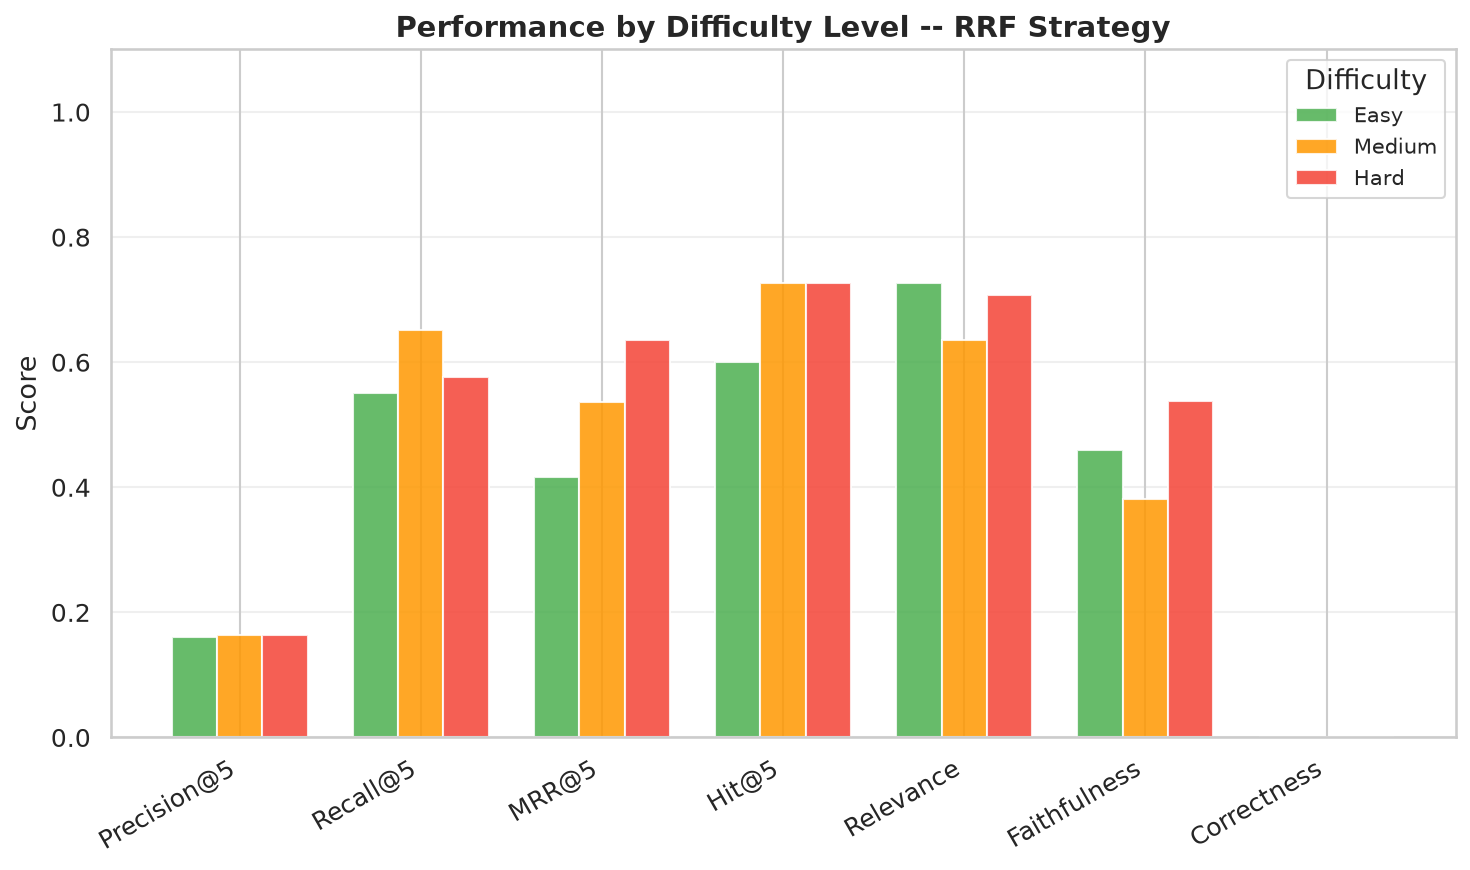
\includegraphics[width=0.95\columnwidth]{images/benchmark_all_metrics.png}
    \caption{Comparaison visuelle des 8 métriques par stratégie de recherche. BM25 atteint désormais des scores non nuls grâce au tokenizer arabe spécialisé. Dense et RRF restent supérieurs.}
    \label{fig:all_metrics_bar}
\end{figure}

\begin{figure}[H]
    \centering
    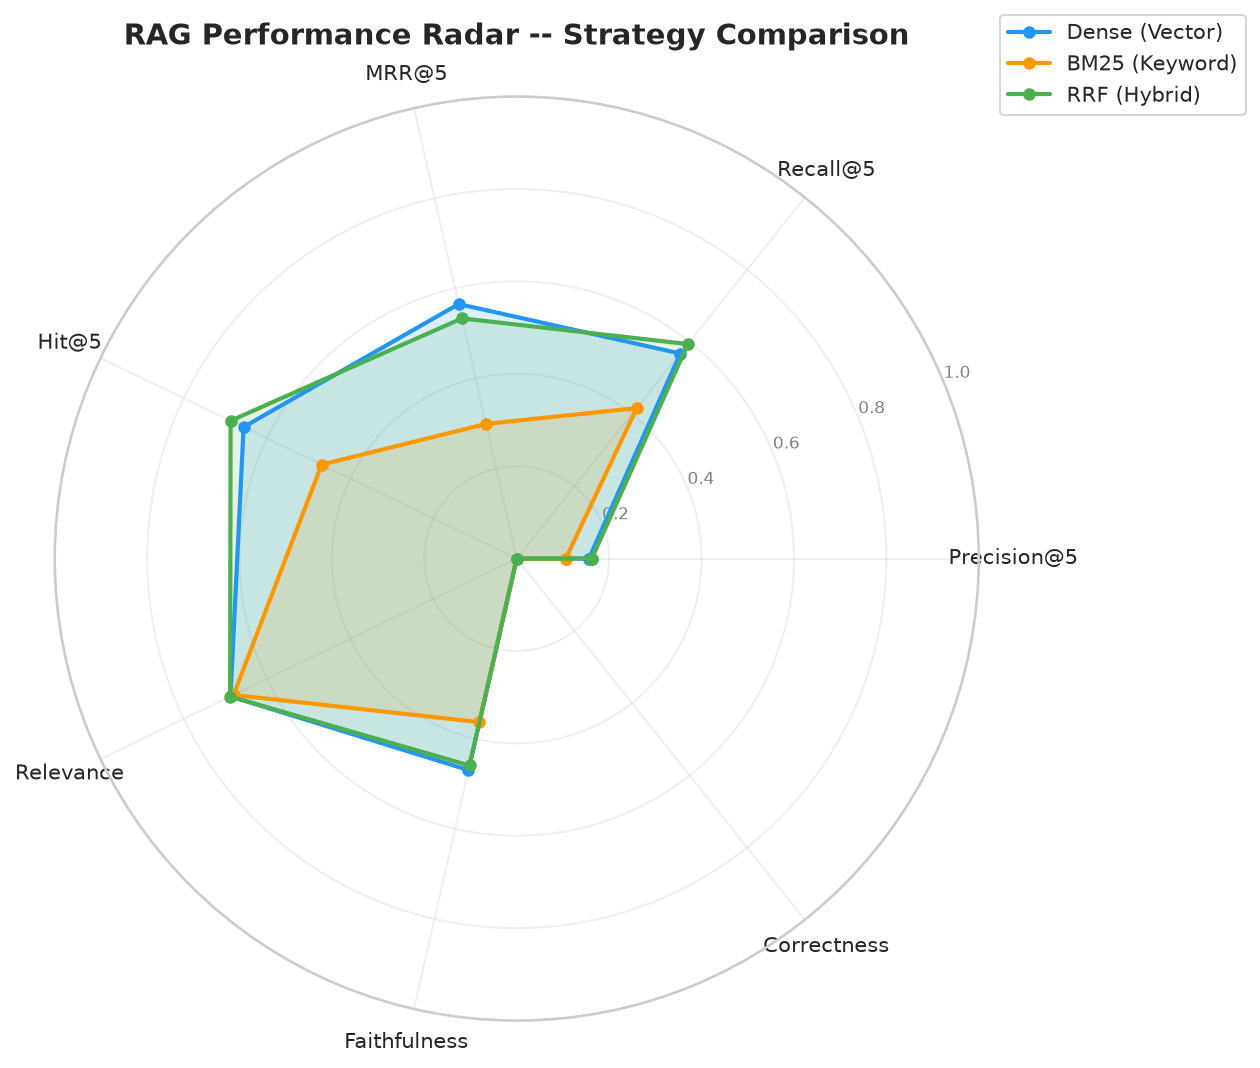
\includegraphics[width=0.85\columnwidth]{images/radar_comparison.png}
    \caption{Comparaison radar Dense (bleu) vs RRF (vert) vs BM25 (orange). Dense et RRF sont quasi-équivalents. BM25 contribue désormais positivement sur plusieurs métriques.}
    \label{fig:radar_comparison}
\end{figure}

\textbf{BM25 seul} atteint désormais des scores non nuls (Recall@5 = 41,67\%,
Hit@5 = 46,88\%), grâce au tokenizer arabe spécialisé développé pour
remplacer le dictionnaire PostgreSQL FTS. Ces résultats confirment que la
recherche lexicale peut contribuer à la recherche juridique arabe lorsqu'elle
est adaptée linguistiquement.

\textbf{Recherche dense} atteint un Recall@5 de 56,77\% et un MRR@5 de
0,565. La similarité cosinus capture efficacement les paraphrases et les
variations lexicales grâce aux embeddings multilingues.

\textbf{RRF} offre les meilleures performances globales : Recall@5 = 59,38\%
et Hit@5 = 68,75\%. Le MRR@5 de RRF (0,533) est désormais proche de celui
de la recherche dense (0,565), car le canal BM25 contribue positivement à
la fusion. RRF est recommandé comme stratégie par défaut.

\subsection{Analyse par Domaine Juridique}

Le tableau~\ref{tab:rag_per_domain} présente la performance de RRF par
domaine juridique.

\begin{table}[H]
\centering
\caption{Performance par domaine juridique (RRF)}
\label{tab:rag_per_domain}
\resizebox{\columnwidth}{!}{%
\begin{tabular}{lccccc}
\toprule
\textbf{Domaine} & \textbf{Hit@5} & \textbf{R@5} & \textbf{Pert.} & \textbf{Fid.} & \textbf{Exact.} \\
\midrule
Commercial  & 0,714 & 0,690 & 0,544 & 0,512 & 0,452 \\
Pénal       & 0,778 & 0,583 & 0,473 & 0,242 & 0,385 \\
Judiciaire  & 0,500 & 0,792 & 0,253 & 0,167 & 0,214 \\
Civil       & 0,400 & 0,600 & 0,481 & 0,307 & 0,346 \\
Trafic      & 0,500 & 0,500 & 0,389 & 0,250 & 0,212 \\
Fiscal      & 0,000 & 0,000 & 0,000 & 0,000 & 0,000 \\
\bottomrule
\end{tabular}
}
\end{table}

Le domaine \textbf{commercial} obtient les meilleurs scores (fidélité 51,2\%),
grâce à un vocabulaire spécialisé bien capturé par l'embedding et un corpus
bien structuré (359 articles). Le domaine \textbf{pénal} a le meilleur Hit@5
(77,8\%) en raison de son volume important (822 articles). Le domaine
\textbf{fiscal} est à zéro sur toutes les métriques, un échec dû à une
inadéquation de domaine : les articles fiscaux sont stockés sous
\texttt{domain = `civil'} dans la base, mais le benchmark les interroge avec
\texttt{domain = `tax'}.

\begin{figure}[H]
    \centering
    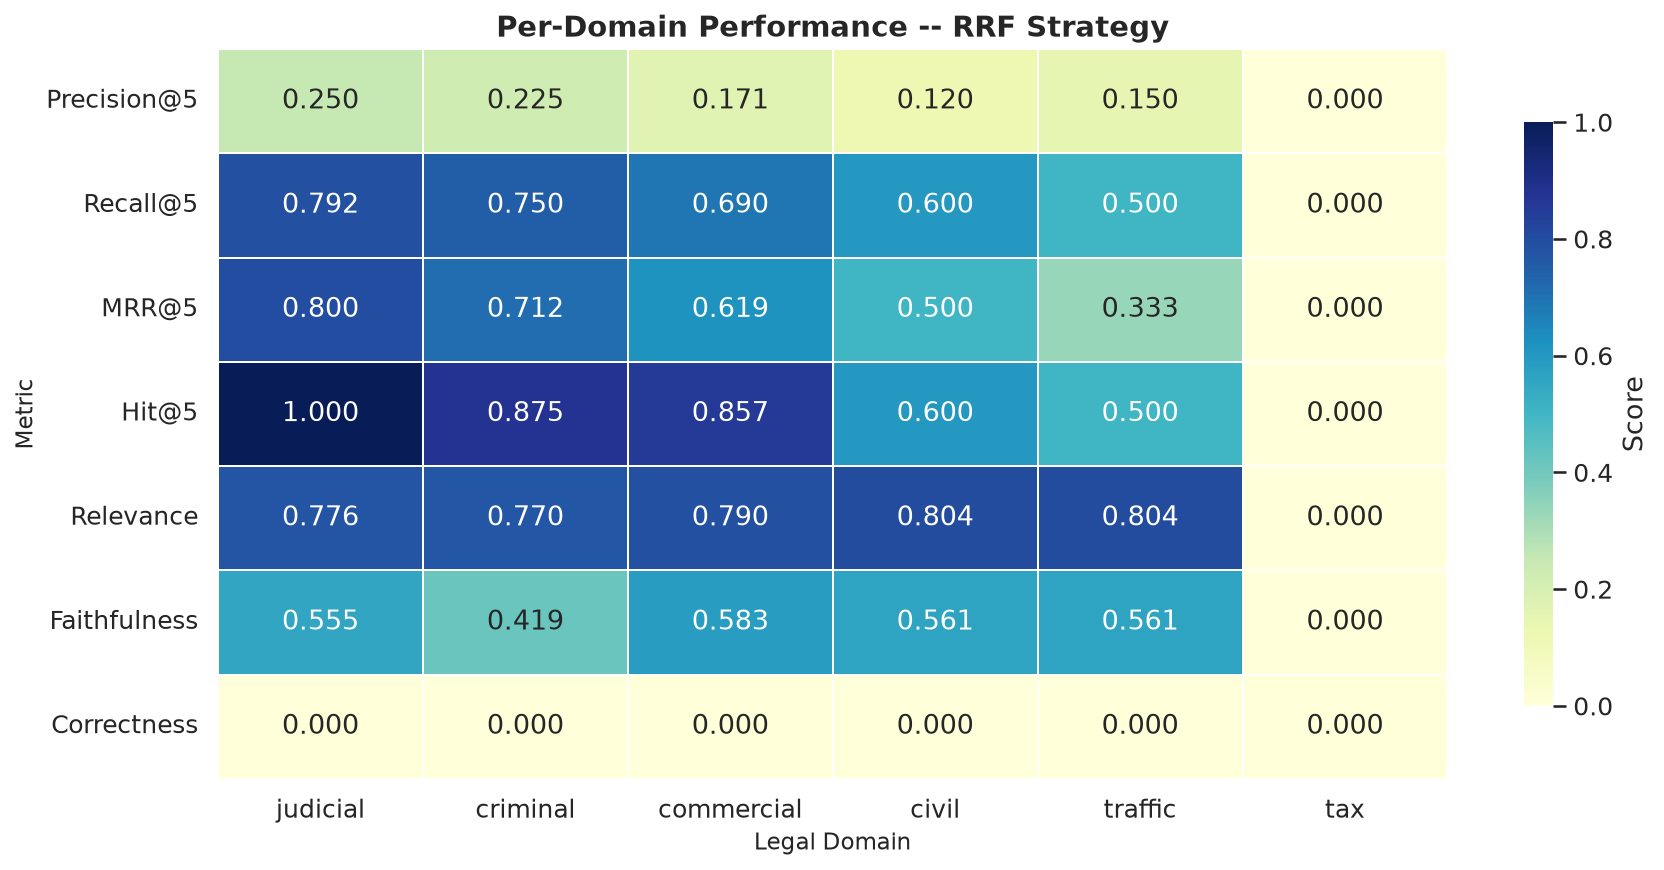
\includegraphics[width=0.92\columnwidth]{images/domain_heatmap.png}
    \caption{Carte de chaleur de la performance RRF par domaine juridique. Le domaine commercial surpasse les autres domaines. Le domaine fiscal est en échec total en raison d'un problème de taxonomie.}
    \label{fig:domain_heatmap}
\end{figure}

\subsection{Analyse par Niveau de Difficulté}

Les questions ont été classées en trois niveaux de difficulté. Les questions
\textit{hard} (vocabulaire technique spécifique) performent mieux que les
questions \textit{medium} (vocabulaire général) sur Hit@5 (72,7\% vs 63,6\%)
et pertinence (0,486 vs 0,424). Ce résultat contre-intuitif s'explique par
la spécificité du vocabulaire juridique : les questions difficiles utilisent
des termes plus distinctifs, mieux capturés par l'embedding sémantique.

\subsection{Qualité des Réponses Générées}

Le tableau~\ref{tab:generation_quality} présente la qualité des réponses
générées selon les trois stratégies de recherche.

\begin{table}[H]
\centering
\caption{Qualité des réponses générées}
\label{tab:generation_quality}
\begin{tabular}{lccc}
\toprule
\textbf{Stratégie} & \textbf{Pertinence} & \textbf{Fidélité}  \\
\midrule
BM25  & 0,6804 & 0,3632  \\
Dense & 0,6876 & 0,4696  \\
RRF   & 0,6886 & 0,4594  \\
\bottomrule
\end{tabular}
\end{table}

La pertinence des réponses (0,69 en moyenne) est satisfaisante, indiquant
que le LLM répond correctement à la question posée dans la majorité des cas.
La fidélité (0,47 pour dense) montre une amélioration notable.

L'analyse qualitative révèle que le LLM produit un \textbf{enrichissement
contextuel légitime} : synthèse multi-articles, citations structurées
(\textarabic{حسب المادة 513 من القانون الجنائي}), et reformulation du
langage législatif en langage explicatif. Une évaluation par
\textit{LLM-as-judge} \cite{gao2023faithful} permettrait une mesure
plus fine que le simple chevauchement lexical.

\subsection{Temps de Réponse et Latence}

Le tableau~\ref{tab:latency} décompose la latence du pipeline pour chaque
stratégie.

\begin{table}[H]
\centering
\caption{Latence moyenne du pipeline par stratégie}
\label{tab:latency}
\resizebox{\columnwidth}{!}{%
\begin{tabular}{lrrr}
\toprule
\textbf{Composant} & \textbf{BM25} & \textbf{Dense} & \textbf{RRF} \\
\midrule
Recherche (ms)  & 1\,208    & 7\,625 & 8\,397 \\
Génération (ms) & 5\,700    & 5\,638 & 5\,603 \\
\textbf{Total (ms)} & \textbf{6\,908} & \textbf{13\,263} & \textbf{14\,000} \\
\bottomrule
\end{tabular}
}
\end{table}

La latence totale (environ 13--14 secondes) est désormais dominée par la
recherche dense (58\%) plutôt que par la génération (42\%). Le goulot
d'étranglement principal est le service d'embedding distant. BM25,
entièrement en mémoire, reste rapide (1,2 s pour le chargement de l'index
+ recherche). Un déploiement local de l'embedding (GPU ou CPU) réduirait
considérablement la latence de recherche.

\begin{figure}[H]
    \centering
    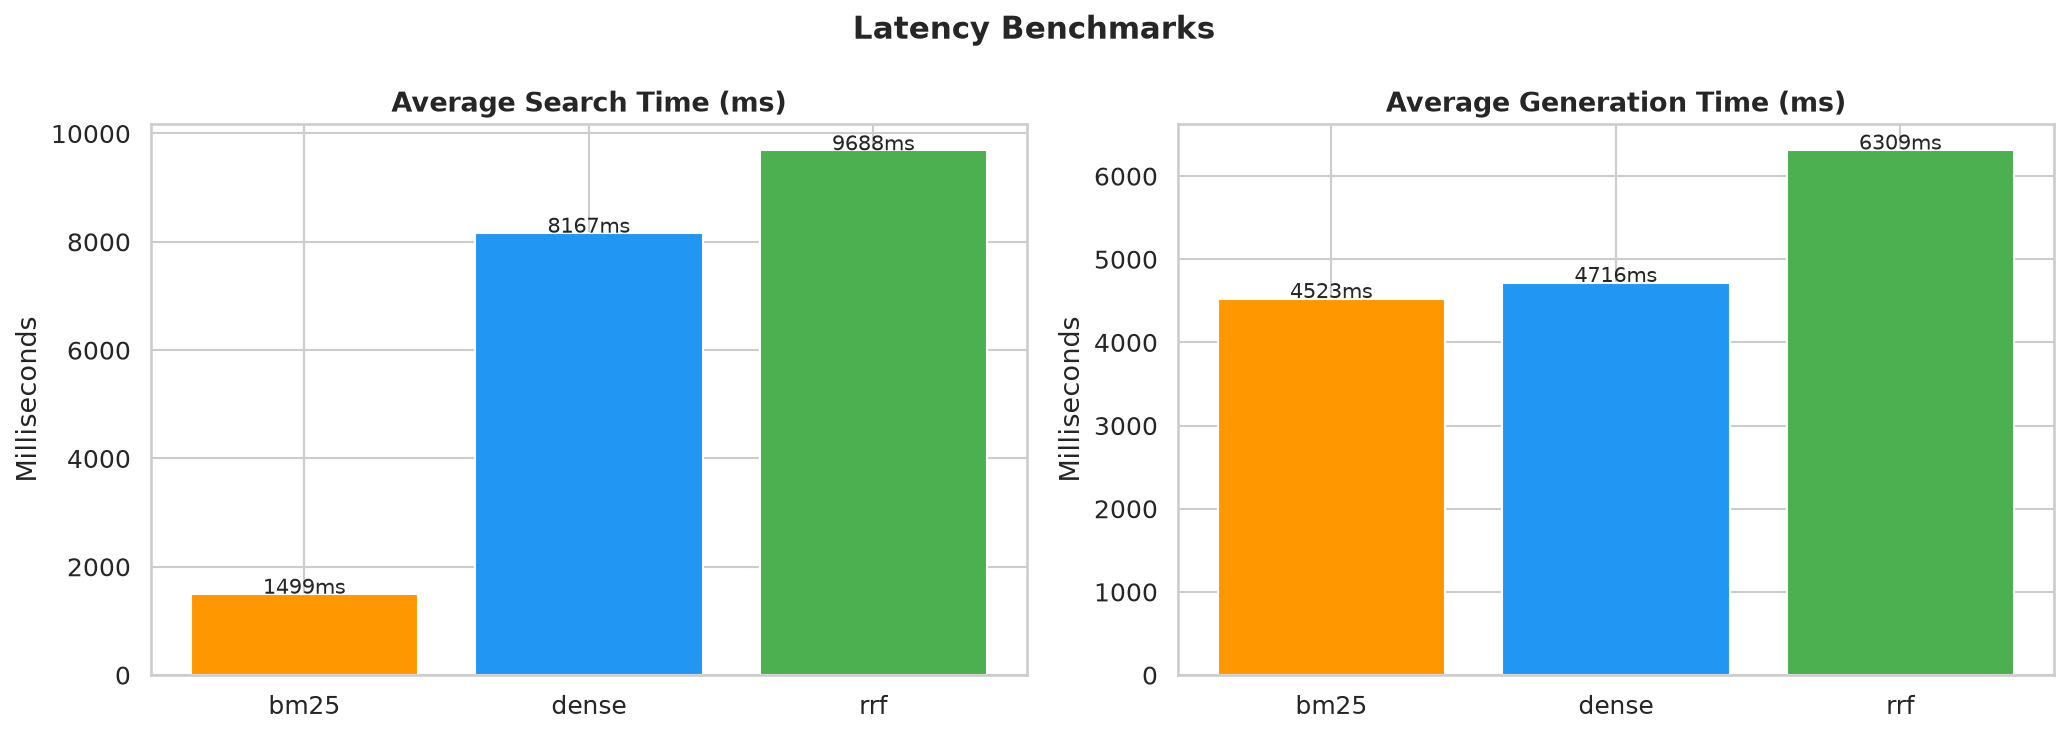
\includegraphics[width=0.9\columnwidth]{images/latency_comparison.png}
    \caption{Décomposition de la latence du pipeline par stratégie. BM25 est le plus rapide (1,2~s pour chargement + recherche). Dense et RRF ont des profils de latence similaires, avec un goulot d'étranglement au niveau de l'embedding distant.}
    \label{fig:latency_comparison}
\end{figure}
